\section{Method}
\label{sec:method}

\begin{figure*}[t]
\centering
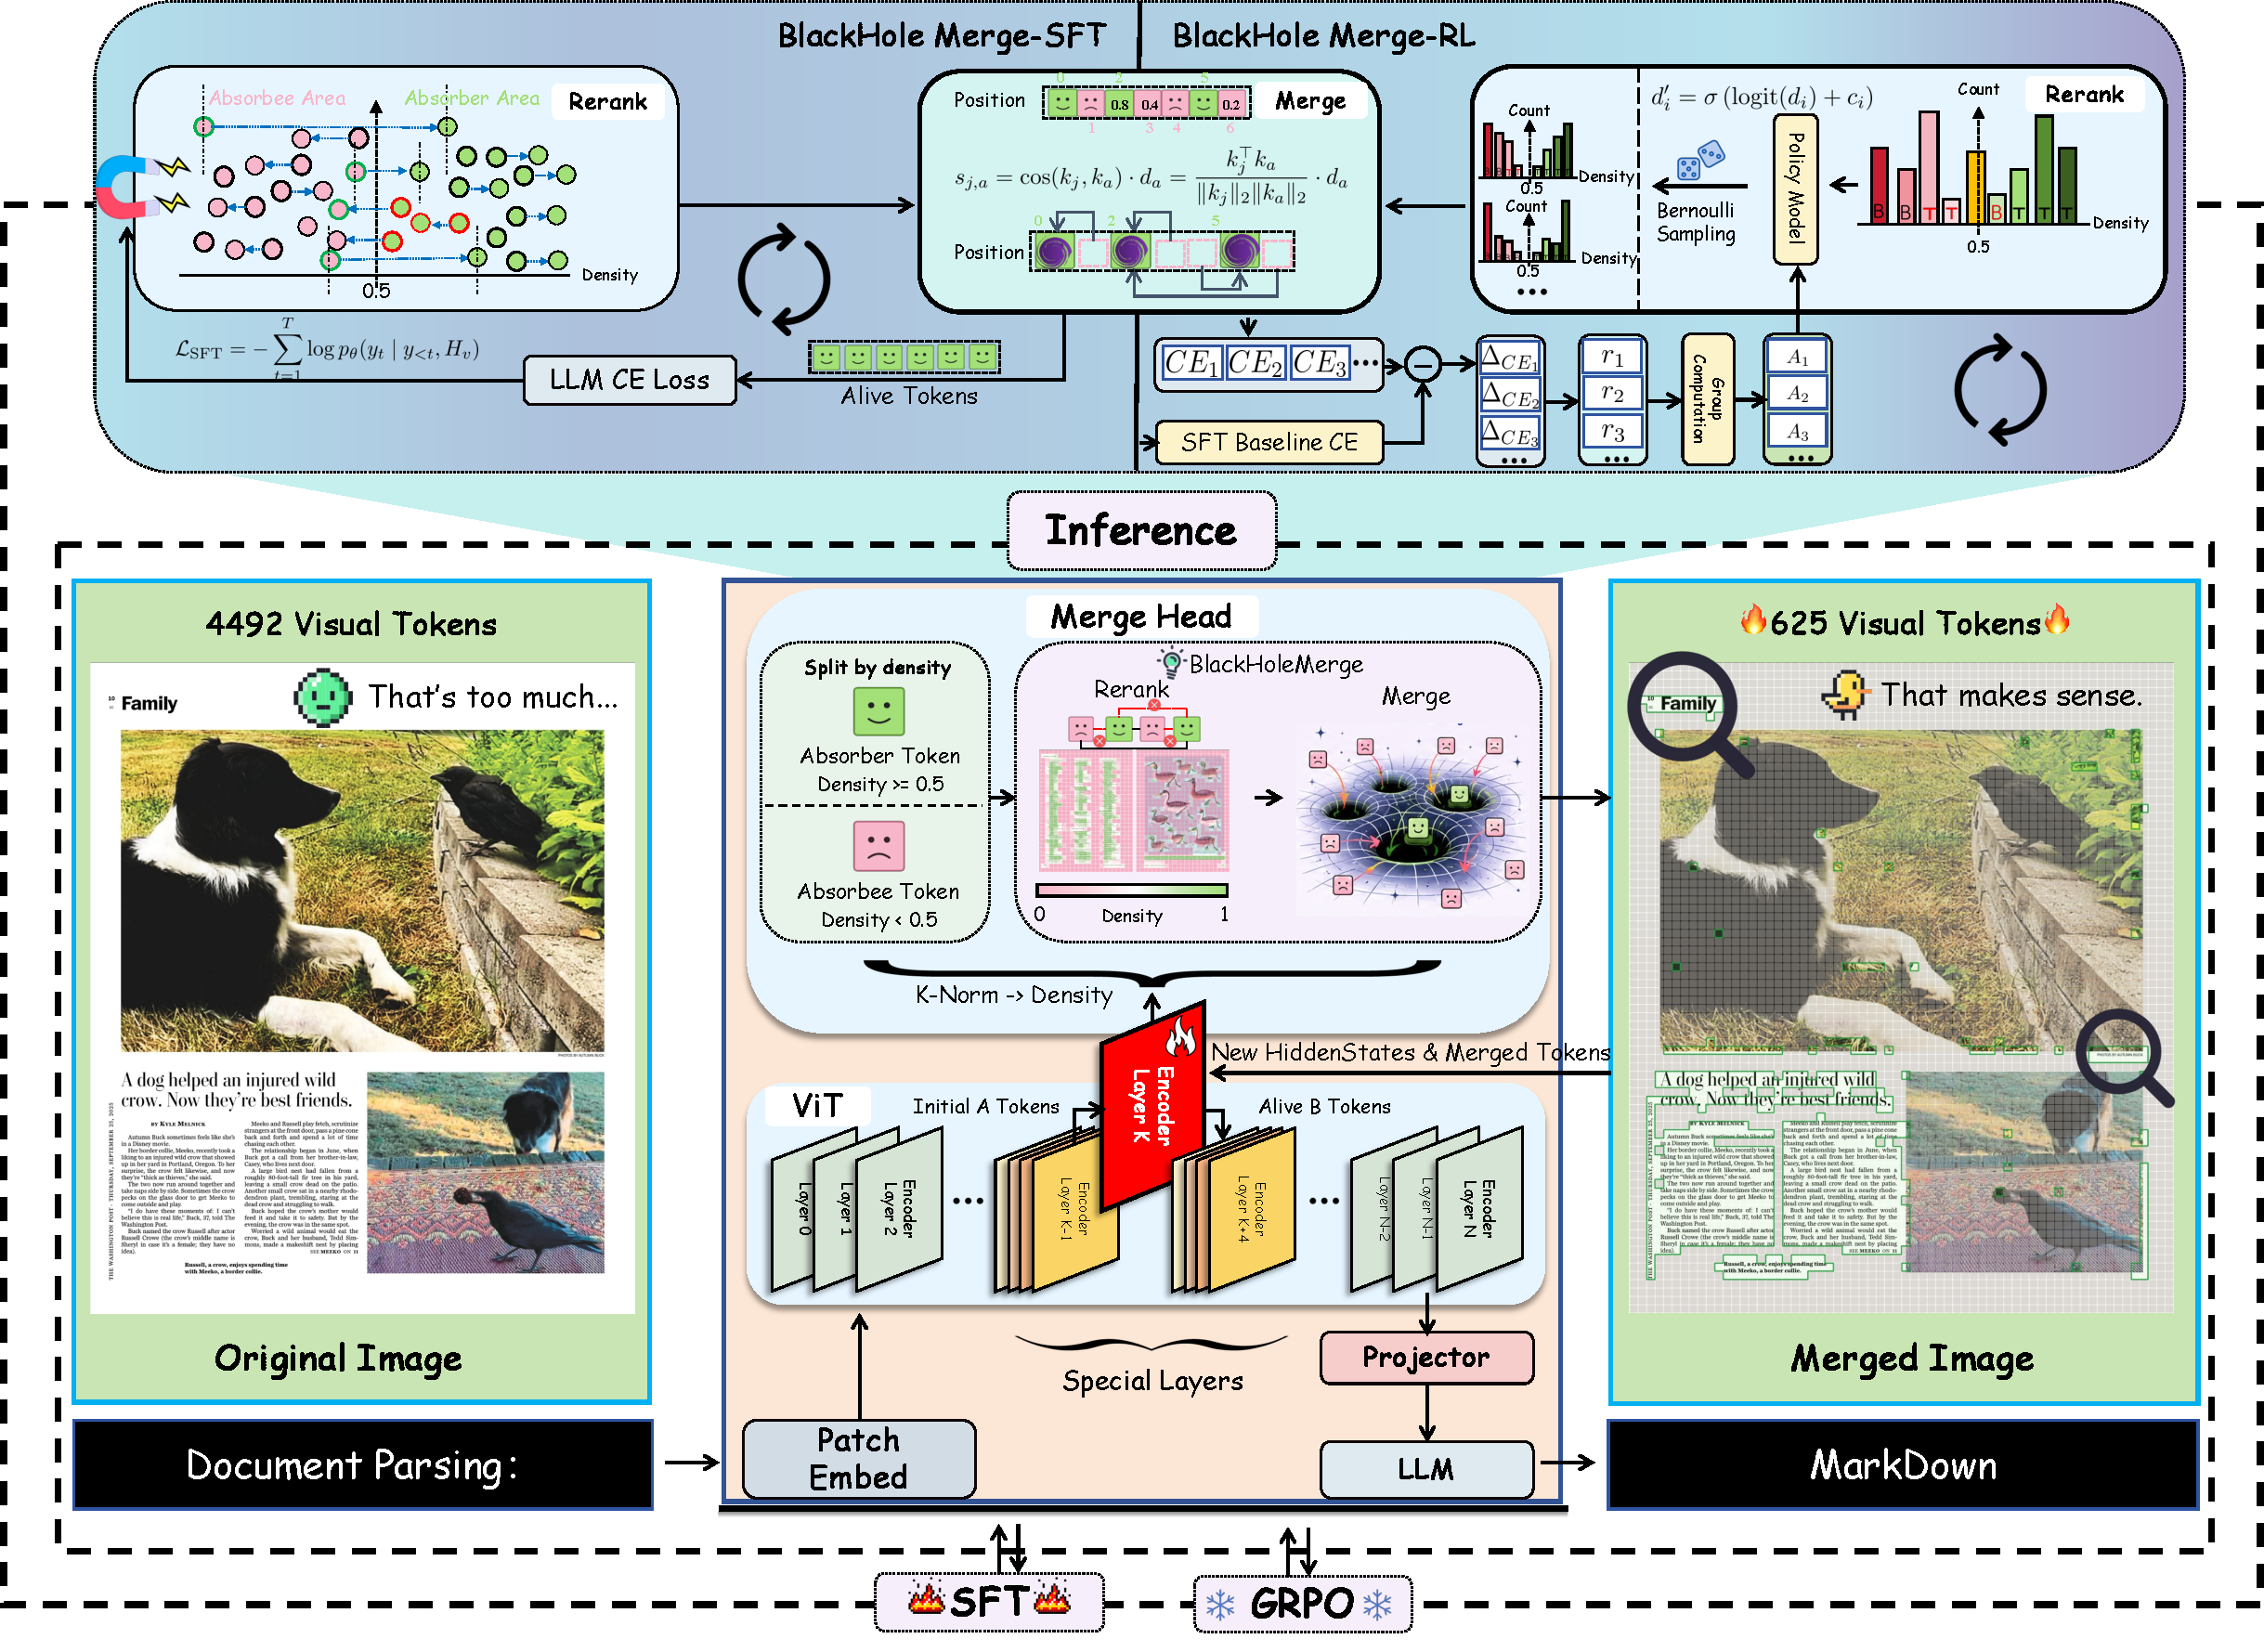
\includegraphics[width=0.9\linewidth]{figures/final/model_arch.pdf}
\caption{Overview of \ours{}. A merge head is inserted at an intermediate ViT layer to keep high-density tokens and merge low-density tokens according to Key-vector density and similarity. Merge-aware SFT and lightweight RL refine the density boundary for stable content-adaptive compression.}
\label{fig:model_arch}
\end{figure*}

\subsection{Overview}

Figure~\ref{fig:model_arch} illustrates the layered compression framework of \ours{}. The lower part of the figure corresponds to the inference pipeline. A document image is first patch-embedded into 4492 visual tokens and then processed by the first half of the ViT ($0\sim k-1$ layers) for contextual modeling. Compression does not happen at the end of the encoder; instead, it is inserted into an intermediate bottleneck at layer $k$. At this merge head, the L2 norm of the current-layer Key vectors is used to estimate token density, and an initial threshold of 0.5 splits tokens into a retained side and a merged side. High-density tokens are kept as absorbers, while low-density tokens are merged into these representative tokens according to K-vector similarity. As a result, the sequence is substantially compressed before entering the second half of the ViT ($k+1\sim N$ layers). In the example shown in the figure, 4492 tokens are reduced to 625 active tokens before being passed to the projector and the LLM for structured OCR generation.

The upper part of the figure corresponds to the training pipeline. SFT and RL jointly learn the same compression bottleneck and progressively stabilize the density boundary: SFT is trained over the full model so that text tokens are more likely to move to the absorber side, making the boundary better aligned with OCR utility; RL then freezes the backbone and trains only a lightweight policy model, further sharpening the keep/drop decisions on top of the SFT baseline CE so that low-priority regions are more consistently assigned to the absorbee side. The detailed training procedure will be further explained in the following subsections.

\subsection{BlackHole Merge}

\subsubsection{K-norm Density Estimation.}

In ViT self-attention, input tokens $X\in\mathbb{R}^{N\times D}$ are projected into
\begin{equation}
Q=XW_Q, \quad K=XW_K, \quad V=XW_V .
\end{equation}

Attention weights are computed by $\mathrm{softmax}(QK^\top/\sqrt{d_k})$. Since Key vectors determine how strongly tokens can be matched in dot-product attention, their norms provide an empirical signal for token content density. We verify this signal across 1,000 OCR documents spanning diverse page types, including newspapers, academic papers, PPT slides, and other document images. As shown in Table~\ref{tab:cross_model_knorm}, text regions consistently have higher K-norms than background regions over continuous visual layers. This suggests that K-norm separation is a common representation pattern rather than an artifact of one model.

\begin{table}[!htbp] 
    \centering
    \fontsize{8}{9}\selectfont
    \renewcommand{\arraystretch}{1.1}
    \setlength{\tabcolsep}{4pt}
    \begin{tabular*}{\columnwidth}{c c c c @{\extracolsep{\fill}}}
        \toprule
        \textbf{Model} & \textbf{Encoder Layers} & \textbf{Span} & \textbf{Best Layer / Gap} \\
        \midrule
        PaddleOCR-VL-1.5 & 27 & 0--25 & 6 / 1.46 \\
        PaddleOCR-VL-1.6 & 27 & 0--25 & 6 / 1.41 \\
        ABot-OCR         & 24 & 0--23 & 8 / 0.66 \\
        FireRed-OCR      & 24 & 0--23 & 8 / 0.66 \\
        dots.ocr         & 42 & 27--41& 32 / 0.63 \\
        Dolphin-1.5      & 20 & 5--19 & 13 / 0.67 \\
        HunyuanOCR       & 27 & 12--26& 18 / 0.73 \\
        MinerU2-VLM      & 26 & 14--25& 20 / 0.57 \\
        \bottomrule
    \end{tabular*}
    \caption{K-norm separation between text and background regions across OCR/document VLMs on 1,000 documents. Gap is defined as $(\operatorname{mean}(K_{\text{text}})-\operatorname{mean}(K_{\text{blank}}))/\operatorname{std}(K_{\text{all}})$. Span denotes the longest continuous layer interval with positive average Gap, and Best denotes the layer with the maximum average Gap.}
    \label{tab:cross_model_knorm}
\end{table}

For token $i$ at the compression layer, the raw density is
\begin{equation}
r_i=\|k_i\|_2 .
\end{equation}
To make densities comparable across pages, we normalize the K-norms within each image by z-score normalization and then map them to $[0,1]$ with a sigmoid:
\begin{equation}
z_i=\frac{r_i-\mu_r}{\sigma_r}, \quad d_i=\sigma(z_i),
\end{equation}
where $\mu_r$ and $\sigma_r$ are the mean and standard deviation of the K-norms in the current image. Here, $z_i=0$ means that token $i$ has the image-level average K-norm, and the sigmoid maps this midpoint to $d_i=0.5$. Therefore, $d_i=0.5$ serves as a natural per-image boundary between higher-than-average and lower-than-average token density. Leveraging this property, we aim to shift the density distribution of text tokens to the right of 0.5, so that they are more likely to be retained as absorbers. 

\subsubsection{Absorber-based Token Merging.}

Given the density $d_i$, tokens are split into absorbers and absorbees:
\begin{equation}
\mathcal{A}=\{i\mid d_i\geq0.5\},\quad
\mathcal{B}=\{i\mid d_i<0.5\}.
\end{equation}

Absorbees are not discarded, since they may still contain useful layout or background context. Instead, each absorbee is merged into one retained absorber. For an absorbee $j\in\mathcal{B}$, we denote its target absorber by $a^*$. We select $a^*$ from $\mathcal{A}$ using density-weighted K-vector similarity:
\begin{equation}
a^*=\arg\max_{a\in\mathcal{A}}
\frac{k_j\cdot k_a}{\|k_j\|\|k_a\|}\cdot d_a .
\end{equation}
Here, the cosine term measures feature compatibility between the absorbee and candidate absorber, while $d_a$ favors high-density absorbers as more reliable representatives.

Because RoPE positional information is injected into Key vectors, the assignment reflects both feature similarity and spatial proximity. We use Key vectors only for absorber assignment; the representations actually merged and passed to later ViT layers are hidden states.

For each absorber $a$, let $\mathcal{B}_a$ denote the set of absorbees assigned to it. We update its hidden state by aggregating low-density residuals, where $d_j<0.5$ for all $j\in\mathcal{B}_a$:

\begin{equation}
\hat{h}_a=h_a+\sum_{j\in\mathcal{B}_a}d_j\cdot(h_j-h_a),
\end{equation}

Thus, each absorbee contributes only a density-weighted residual toward the absorber, and lower-density tokens have weaker influence. This keeps the retained absorber as the dominant representation while still preserving part of the compressed contextual information. After merging, the visual hidden states are reduced from $N$ to ${A}$, and the compression ratio adapts to page content.

To further visualize the merging behavior of BlackHole Merge, we count how many tokens are absorbed by each spatial location and normalize the counts within each image, resulting in the heatmap shown in Fig.~\ref{fig:absorb_all}. We observe that dense text regions usually absorb fewer tokens, whereas text boundaries and text-background interfaces absorb the most. This is because boundary tokens are more similar to surrounding blank regions and carry less independent semantic information, making them natural absorption points for low-density tokens. This result indicates that \ours{} does not uniformly push all background information into text cores; instead, it prefers to compress locally at text boundaries, which is consistent with the spatial distribution of information density in document pages.

\begin{figure}[t]
\centering
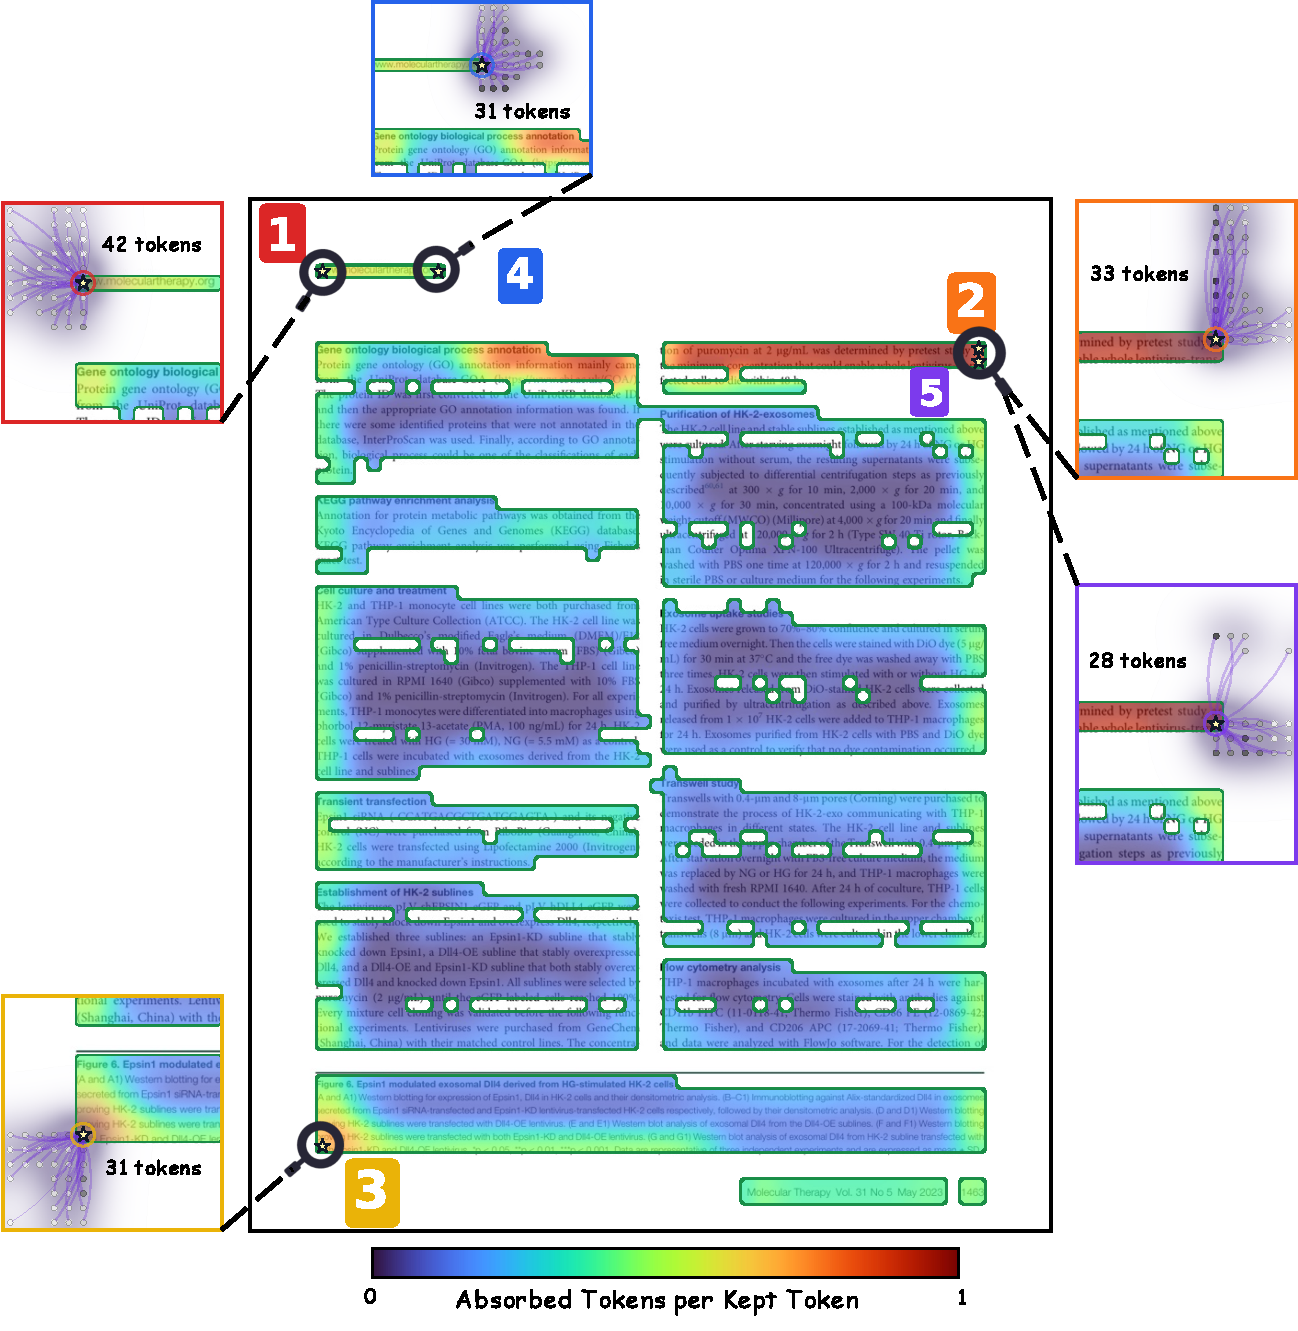
\includegraphics[width=\linewidth]{figures/final/absorbtion_all.pdf}
\caption{Token absorption heatmap of \ours{}. Colors indicate the normalized number of absorbees assigned to each retained token. Most absorptions occur around text boundaries and text-background interfaces, showing that low-density background tokens are compressed through locally similar representatives rather than merged into text cores.}
\label{fig:absorb_all}
\end{figure}

\subsection{Training and Inference}

\subsubsection{Merge-aware SFT.}

In the first stage, BlackHole Merge is enabled during supervised fine-tuning and trained end-to-end over the full model. SFT does more than teach the model to perform OCR on compressed sequences; it also reorders the density ranking induced by K-norm. As shown in Fig.~\ref{fig:model_arch}, the black-outlined circles denote tokens whose density ranking remains essentially stable before and after SFT, whereas the red/green concentric circles denote tokens whose relative ranking changes. Such changes are not restricted to tokens near the decision boundary. Since density is normalized within each image, the SFT objective induces a global re-ranking effect: changes in one token's relative importance can affect the ordering of many others. This is why SFT can rapidly reduce CE while pushing OCR-relevant tokens toward the absorber side and background tokens toward the absorbee side.

However, this effect is only coarse. Once the main text regions are separated, optimization tends to saturate. SFT may continue to suppress some background tokens, but it is not sufficient to further tighten the boundary, which motivates RL for finer refinement. To prevent the CE loss from directly manipulating density weights and weakening compression, we stop the gradient of each absorbee density:
\begin{equation}
h_{a^*}\leftarrow h_{a^*}+\mathrm{sg}(d_j)\cdot(h_j-h_{a^*}).
\end{equation}

Here, $\mathrm{sg}(d_j)$ only controls the forward merging strength, while gradients mainly update the ViT hidden states and Key representations. In other words, CE loss cannot directly increase or decrease density weights; it can only reshape the hidden states and Key representations, which then changes the density ranking in later forward passes. After SFT, the density distribution becomes more aligned with OCR utility: many text and structural tokens move toward the absorber side, while many blank and repetitive background tokens move toward the absorbee side.

However, SFT still produces an uncertain boundary. As shown in Fig.~\ref{fig:sft_curve}, the visualization contains three views: the original token layout, the SFT-compressed token layout, and the resulting density histogram. Although SFT reduces the number of visual tokens and moves many OCR-relevant tokens to the absorber side, the density histogram remains scattered, with many tokens still falling into the gray zone around $0.3$--$0.6$. This indicates that the keep/merge decision is not yet confident enough. Therefore, merge-aware SFT provides a coarse content-aware ranking, while the following RL stage is needed to further polarize the density distribution and sharpen the boundary.

\begin{figure}[!htbp]
\centering
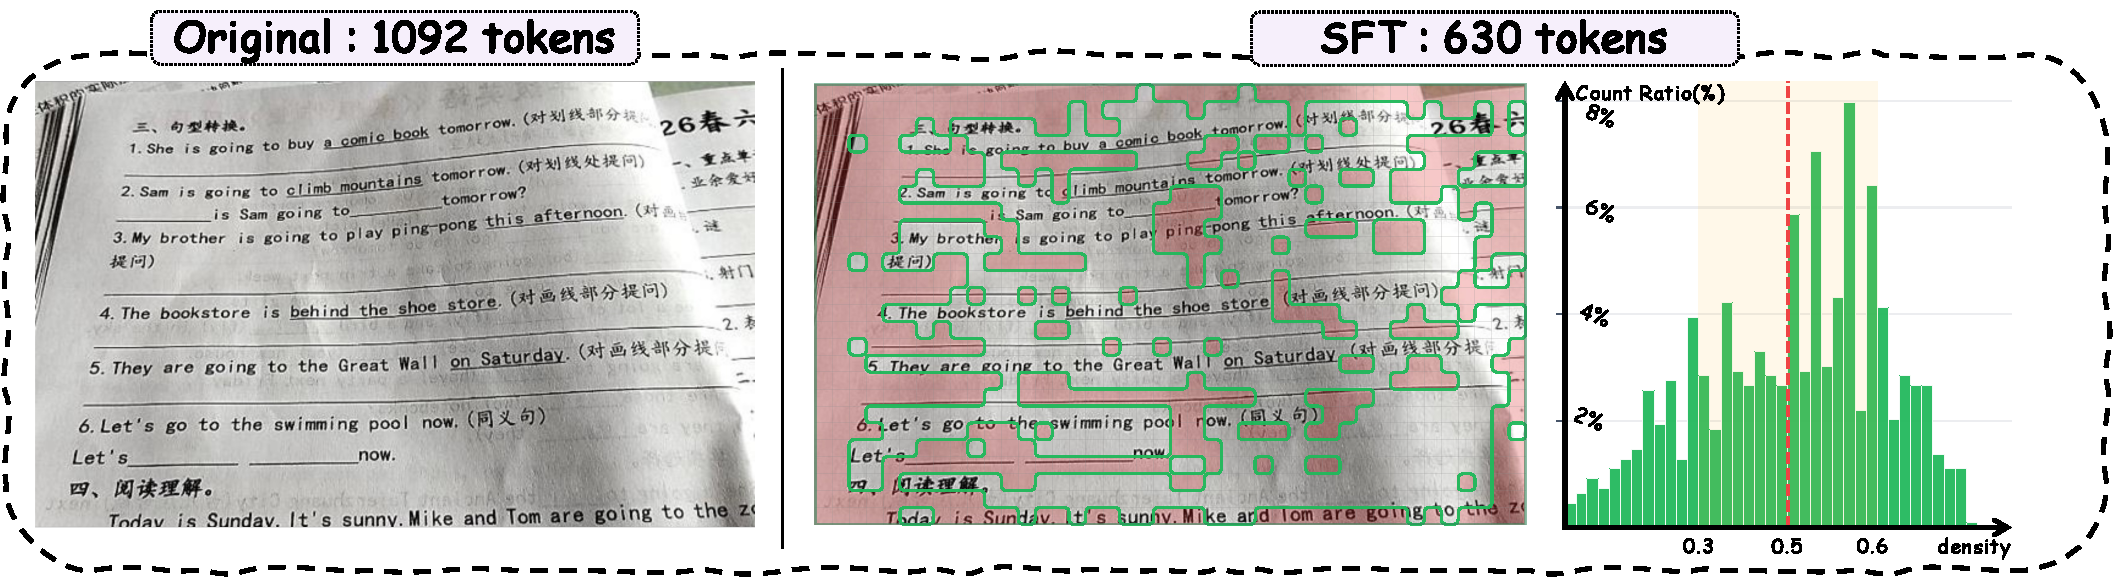
\includegraphics[width=\linewidth]{figures/final/wanqu_sft.pdf}
\caption{Effect of merge-aware SFT. The figure shows the original token layout, the SFT-compressed layout, and the resulting density histogram. SFT reduces visual tokens and aligns density with OCR utility, but many tokens remain in the gray zone around $0.3$--$0.6$, indicating that the keep/merge boundary is still uncertain.}
\label{fig:sft_curve}
\end{figure}

\subsubsection{Lightweight RL Policy.}
As shown in the upper-right part of Fig.~\ref{fig:model_arch}, in the second stage we freeze the ViT, projector, and LLM, and train only a lightweight policy MLP. This stage does not relearn visual representations; instead, it refines the keep/drop boundary on top of the density ordering learned by SFT. Given the full Key vector $k_i$ of the $i$-th token, the policy predicts a logit-space correction:
\begin{equation}
\mathrm{correction}_i=\mathrm{MLP}(k_i) .
\end{equation}
\begin{equation}
d_i'=\sigma\left(\mathrm{logit}(d_i)+\mathrm{correction}_i\right).
\end{equation}
The adjusted density $d_i'$ still represents the token retention tendency. Since the policy observes the full Key vector, it can exploit directional information beyond the Key norm and distinguish tokens with similar norms but different semantics, thereby reducing the ambiguous gray zone left by SFT, defined as tokens with $0.3<d<0.6$.

We train the policy with GRPO. For each sample, we draw $K=8$ keep/drop masks from the current $d_i'$ and evaluate each compressed sequence with teacher-forcing CE after BlackHole Merge. Instead of using the uncompressed input as the reference, we use the CE under the SFT hard mask as the baseline:
\begin{equation}
\mathrm{CE}_{\mathrm{base}}
=\mathrm{TeacherForcing}(\mathrm{SFT\ hard\ mask},\mathrm{GT}).
\end{equation}
This restricts RL to improve the compression boundary around the operating point already adapted by SFT, rather than competing with an uncompressed upper bound.

For each group of rollouts, GRPO updates the policy with group-relative advantages:
\begin{equation}
\mathcal{L}_{\mathrm{GRPO}}
=-\frac{1}{K}\sum_{k=1}^{K}
A_k\log \pi_\theta(m_k\mid d'),
\end{equation}
where $m_k$ is the $k$-th sampled mask and $A_k$ is its relative advantage within the group. We construct $A_k$ according to the CE change against the SFT baseline. Let
\begin{equation}
\Delta\mathrm{CE}_k=\mathrm{CE}_{\mathrm{base}}-\mathrm{CE}_k .
\end{equation}
If $\Delta\mathrm{CE}_k\geq0$, the rollout does not degrade teacher-forcing quality. In this case, we compare only the safe rollouts and assign larger positive advantages to masks with higher compression. With $c_k$ denoting the compression ratio,
\begin{equation}
A_k=\mathrm{Norm}_{\mathcal{G}_{\mathrm{safe}}}(c_k),
\qquad k\in\mathcal{G}_{\mathrm{safe}} .
\end{equation}
If $\Delta\mathrm{CE}_k<0$, the rollout hurts output quality. It receives a negative advantage, further amplified by the amount of high-confidence SFT tokens it removes:
\begin{equation}
A_k=\Delta\mathrm{CE}_k\left(1+\mathrm{drop\_conf}_k\right),
\qquad k\in\mathcal{G}_{\mathrm{penalty}},
\end{equation}
\begin{equation}
\mathrm{drop\_conf}_k=
\frac{\sum_{i\in\mathcal{S}_{\mathrm{drop}}}(d_i-0.5)}
{\sum_{i\in\mathcal{S}_{\mathrm{sft}}}(d_i-0.5)} .
\end{equation}
Here, $\mathcal{S}_{\mathrm{sft}}$ denotes the tokens retained by the SFT hard mask, and $\mathcal{S}_{\mathrm{drop}}$ denotes the high-confidence tokens additionally removed by the current rollout. This design encourages the policy to pursue higher compression when quality is preserved, while penalizing quality-degrading masks that remove text or structural tokens confidently kept by SFT.

Therefore, GRPO does not require explicit token-level keep/drop labels. It refines the boundary through relative comparison among multiple masks sampled for the same input. SFT provides a task-aware coarse density ordering, and RL sharpens the ambiguous region around this ordering into clearer compression decisions.

Fig.~\ref{fig:rl_curve} further illustrates this refinement process. After RL, the density distribution becomes more polarized than in SFT: tokens originally spread across the middle region are pushed further toward the absorber or absorbee side, the gray zone is substantially reduced, and a cleaner V-shaped distribution emerges. At the same time, more OCR-relevant tokens remain on the absorber side, while background and redundant regions are more stably assigned to the absorbee side. This indicates that RL does not relearn the compression rule from scratch, but rather sharpens the decision boundary on top of the coarse separation established by SFT.

\begin{figure}[!htbp]
\centering
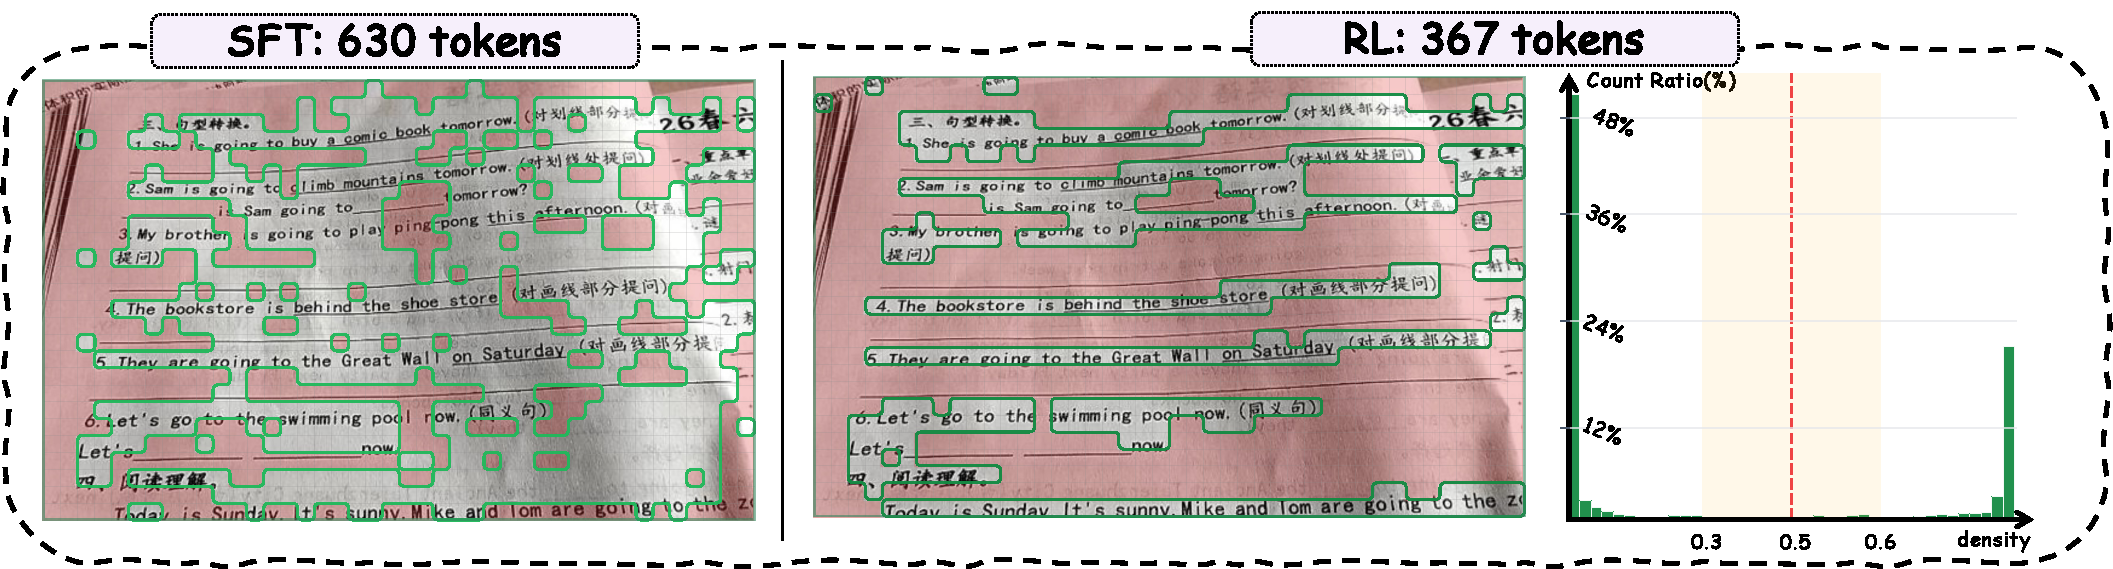
\includegraphics[width=\linewidth]{figures/final/wanqu_rl.pdf}
\caption{RL refinement on the same sample. With the backbone frozen, the policy MLP further compresses the SFT output from 630 to 367 tokens; the density histogram on the right shows a clearer separation and a smaller mid-density region around the 0.5 threshold.}
\label{fig:rl_curve}
\end{figure}

\subsubsection{Inference.}
  At inference time, we directly use the SFT-adapted merge layer
  together with the lightweight Policy MLP trained by GRPO (about 74K
  parameters) for deterministic compression. Specifically, visual
  tokens first obtain density at the merge layer, then the policy
  applies a single forward correction, and the final keep/drop decision
  is made with the threshold $d_i' \geq 0.5$. The compressed visual
  sequence is then passed through the remaining ViT blocks, projector,
  and LLM, and the decoder generates the output autoregressively. No
  GRPO sampling or reward computation is performed during inference, so
  the extra cost is limited to one lightweight density correction pass.

  In terms of computational complexity, BlackHole Merge reduces the
  input length of the subsequent ViT blocks from $N$ visual tokens to
  $M$ retained tokens, so the dominant self-attention cost changes from
  $O(N^2)$ to $O(M^2)$.
  
  The merge step itself only introduces one lightweight density
  correction and token assignment, whose overhead is usually negligible
  compared with the quadratic cost of the later ViT blocks.

  For end-to-end inference time, the main gain comes from the visual
  encoder and the LLM prefill stage, since far fewer visual tokens are
  passed to the projector and the LLM. In contrast, decoder-side
  autoregressive generation is still mainly determined by the output
  length, so its speedup is typically smaller than that of prefill,
  although the overall latency is still reduced. In other words, after
  compression, the main bottleneck shifts from long visual-sequence
  computation to text decoding.

Under the VLM-only setting of PaddleOCR-VL-1.6, we further illustrate the compression effect of BlackHole Merge. Fig.~\ref{fig:overview} shows the visualizations at layer6 and layer9 in two representative cases: one with dense text regions and the other with sparse text regions. In both cases, the results exhibit clear content-adaptive compression:
  text-heavy regions retain more visual tokens, while background and
  redundant regions are merged more aggressively. Meanwhile, the key
  text regions are consistently preserved, indicating that BlackHole
  Merge can stably retain the information required for OCR across
  different layout patterns.
\begin{figure*}[t]
\centering
\begin{minipage}{0.48\linewidth}
\centering
\includegraphics[width=\linewidth]{figures/final/world.pdf}
\end{minipage}
\hfill
\begin{minipage}{0.48\linewidth}
\centering
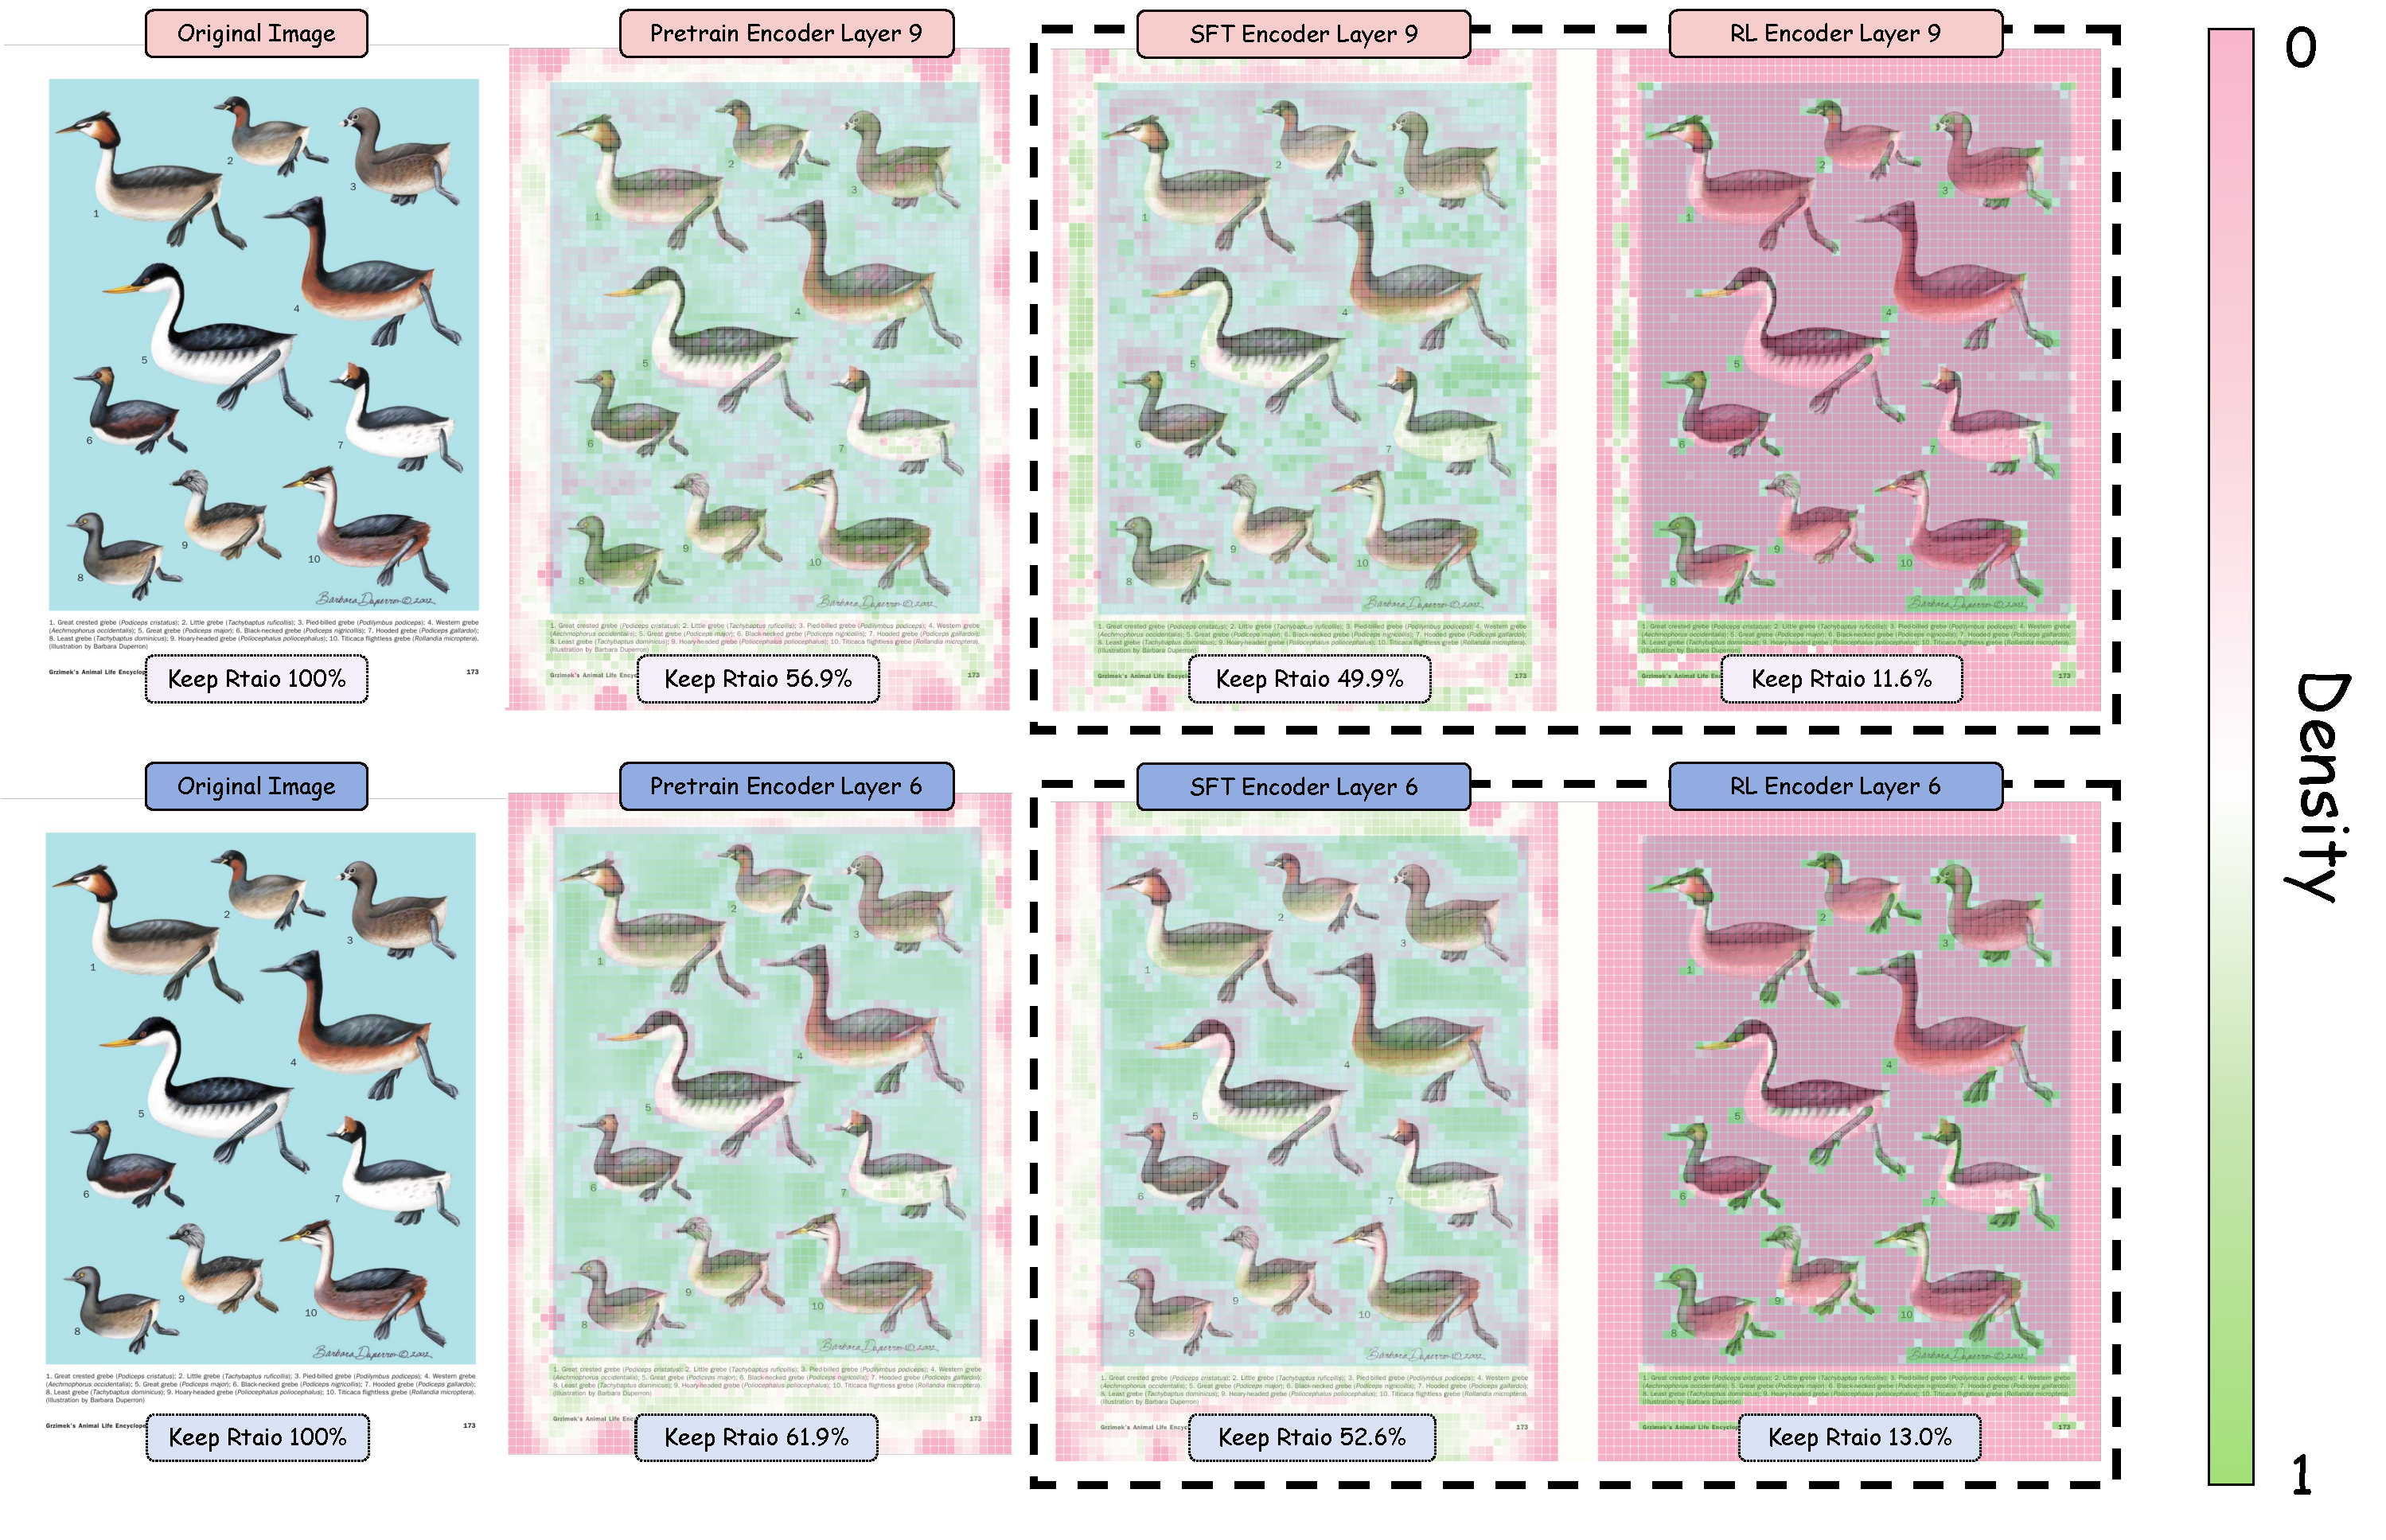
\includegraphics[width=\linewidth]{figures/final/duck.pdf}
\end{minipage}
\caption{Changes in compression decisions of \ours{} from merge-aware SFT to RL post-training. Left: world case; Right: duck case.}
\label{fig:overview}
\end{figure*}
